\documentclass{article}
\usepackage[a4paper,left=2.5cm,right=2.5cm,top=3cm,bottom=2.5cm]{geometry}
\usepackage{ctex}
\usepackage{float}
\usepackage{graphicx}
\usepackage{makecell}
\usepackage{listings}
\usepackage{fontspec}
\usepackage{amsmath}
\setmainfont{Times New Roman}
\usepackage[framed,numbered,autolinebreaks,useliterate]{mcode}
\lstset{language=Matlab,basicstyle=\normalsize}
\pagestyle{empty}
\begin{document}
	\begin{table}
		\begin{figure}[H]
			\centering
			\quad \\[50pt]
			
\includegraphics[width=9.98cm,scale=1.51]{./figures/ico.jpg}
			\quad \\[33.5pt]
		\end{figure}
	\end{table}
	\begin{center}
		\bfseries\heiti\zihao{0}《信号与系统》课程\\[14pt]
		实验报告
	\end{center}
%	\hspace*{\fill} \\[5pt]
	\quad \\*
	\begin{table}[H]
		\centering
		\begin{tabular}[top]{cc}
			\rule{0pt}{25pt}
			\makebox[7em][s]{\songti\zihao{-3}学\hspace{\fill}院}\  & \makebox[16em][s]{\songti\zihao{-3}信息科学与工程学院} \\
			\Xcline{2-2}{1.2pt}
			\rule{0pt}{25pt}
			
			\makebox[7em][s]{\songti\zihao{-3}专\hspace{\fill}业}\  & {\songti\zihao{-3}111} \\
			\Xcline{2-2}{1.2pt}
			\rule{0pt}{25pt}
			
			\makebox[7em][s]{\songti\zihao{-3}班\hspace{\fill}级}\  & {\zihao{-3}x\songti\zihao{-3}xxx} \\
			\Xcline{2-2}{1.2pt}
			\rule{0pt}{25pt}
			
			\makebox[7em][s]{\songti\zihao{-3}学\hspace{\fill}号}\  & {\zihao{-3}xxx} \\
			\Xcline{2-2}{1.2pt}
			\rule{0pt}{25pt}
			
			\makebox[7em][s]{\songti\zihao{-3}姓\hspace{\fill}名}\  & {\songti\zihao{-3}xxx} \\
			\Xcline{2-2}{1.2pt}
			\rule{0pt}{25pt}
			
			\makebox[7em][s]{\songti\zihao{-3}指导教师}\  & {\songti\zihao{-3}xxx} \\
			\Xcline{2-2}{1.2pt}
			\rule{0pt}{41.6pt}
			
			\makebox[7em][s]{\songti\zihao{-3}完成日期}\  & {\songti\zihao{-3}xxx\songti\zihao{-3}年xxx\songti\zihao{-3}月xxx\songti\zihao{-3}日} \\
			\Xcline{2-2}{1.2pt}
		\end{tabular}
	\end{table}
	\newpage
	\begin{center}
		{\heiti\zihao{-2}实验三\quad 连续时间周期信号的傅里叶级数}
	\end{center}
	\setcounter{section}{1}
	\subsection{{\heiti\zihao{4}实验目的}}
	\begin{enumerate}
		\item [(1)] 掌握连续时间周期信号的傅里叶级数的展开和合成,理解吉布斯现象;
		\item [(2)] 掌握周期矩形脉冲信号的频谱及脉冲宽度、周期对周期信号频谱的影响。
	\end{enumerate}
	\subsection{{\heiti\zihao{4}实验原理(或实验方法)}}
	\subsubsection{信号的频谱}
	\subsubsection{矩形脉冲信号的频谱}
	\subsection{{\heiti\zihao{4}实验内容}}
%		源程序(要有,附上必要的注释)\\
%		实验结果(图形)(图形大小、位置适中)\\
%		结果说明或分析
	\begin{enumerate}
		\item[(1)] 周期信号的傅里叶级数的展开和合成
		
		画出如下图对称方波(取$E=1\text{、}T=1$),并采用有限项傅里叶级数对原函数进行逼近,画出对称方波的1、3、5、7、9、11次谐波的傅里叶级数合成波形,观察吉布斯现象。
		\begin{figure}[H]
			\centering
			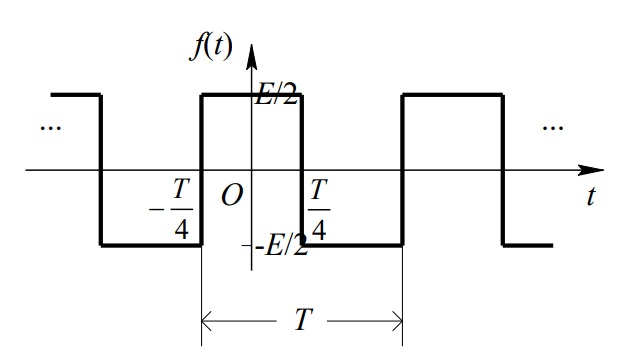
\includegraphics[scale=0.5]{./figures/1.jpg}
			\caption{}
		\end{figure}
		\item[(2)] 周期矩形脉冲信号的频谱结构与波形参数($\tau,T$)之间关系(教材 P81)
		\begin{enumerate}
			\item[(a)] 取$E=1,\tau=1,T=5\tau$画出周期矩形脉冲及其傅里叶级数的频谱(图3-8(b));
			\item[(b)] 取$E=1,\tau=1$,画出图3-8(a);
			\item[(c)] 取$E=1,\tau=1$,画出图3-8(c);
		\end{enumerate}
	\end{enumerate}
	\subsection{{\heiti\zihao{4}思考题}}
	\begin{enumerate}
		\item[(1)] $\frac{\tau}{T}=1/4$的矩形脉冲信号在哪些谐波分量上幅度为零?请画出基波信号频率为5KHz的矩形脉冲信号的频谱图。
		\item[(2)] 要提取一个$\frac{\tau}{T}=1/4$的矩形脉冲信号的基波和2、3次谐波,以及4次以上的高次谐波,可以选用几个什么类型(低通?带通?…)的滤波器?
		\item[(3)] 方波信号在哪些谐波分量上幅度为零?请画出信号频率为2KHz的方波信号的频谱图。
		\item[(4)] 要完整的恢复出原始矩形脉冲信号,各次谐波幅度要成什么样的比例关系?
	\end{enumerate}
	\subsection{{\heiti\zihao{4}实验收获与心得}}
\end{document}